\chapter{OBJETIVOS}
\label{cap:objetivos}

    \section{Objetivos Gerais}
    \label{sec:objetivos-gerais}

       Desenvolver aplicativo funcional que permita a implementação do sistema de autoavaliação do \gls{PPGEEC}.
    \section{Objetivos Específicos}
    \label{sec:objetivos-especificos}
       \begin{alineascomponto}
        	\item Organizar dados, fichas de avaliação e legislação do sistema de autoavaliação do \gls{PPGEEC}.
        	\item Implantar a infra-estrutura para aplicação do sistema de autoavaliação.
        	\item Validar o desenvolvimento do sistema junto aos seus potenciais usuários.
        % 	\begin{subalineascomponto}
        % 		\item Integer non lacinia magna. Aenean tempor lorem tellus, non sodales nisl commodo ut
        % 		\item Proin mattis placerat risus sit amet laoreet.
        % 	\end{subalineascomponto}
        \end{alineascomponto}
        
        %Mais exemplos e opções de citações podem ser encontradas em:
        
%        https://en.wikibooks.org/wiki/LaTeX/Bibliography_Management
%        https://github.com/cfgnunes/latex-cefetmg/blob/master/latex-cefetmg/03-elementos-pos-textuais/apendices.tex        
        
        

%     \section{Inserindo figuras}
%     \label{sec:figuras}
    
%     A Figura \ref{fig:reitoria} apresenta a fotografia da reitoria da Universidade Federal do Ceará. Observe a estrutura do código para inserir a Figura \ref{fig:reitoria}. No título, apenas a primeira letra da frase é maiúscula  exceto nomes próprios e não há ponto final. Procure ajustar o tamanho da figura para preencher a largura delimitada pelas margens esquerda e direita. Não esqueça de indicar fonte da figura. 
    
% \begin{figure}[h!]
%     \Caption{\label{fig:reitoria} Fotografia da Reitoria da Universidade Federal do Ceará}
%     %\centering
%     \UFCfig{}{
%         \fbox{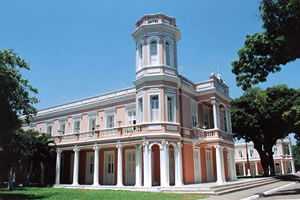
\includegraphics[width=12cm]{figuras/exemplo-1}}
%     }{
%     \Fonte{\citeonline{UFC2012}.}
%     }	
% \end{figure}

% \begin{figure}[!ht]
%     \centering
%     \caption{Fluxograma do experimento do tipo}
%     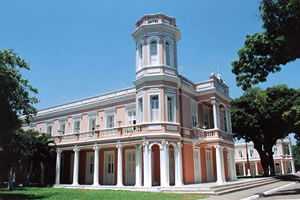
\includegraphics[width=0.9\textwidth]{figuras/exemplo-1}
%     \Fonte{Elaborado pelo autor.}
%     \label{fig:np_np}
% \end{figure}

%     Texto texto texto texto texto texto texto texto texto texto texto texto texto texto texto texto texto texto texto texto texto texto texto texto texto texto texto texto texto texto texto texto texto texto texto texto texto texto texto texto texto texto texto texto texto.

%     Texto texto texto texto texto texto texto texto texto texto texto texto texto texto texto texto texto texto texto. Texto texto texto texto texto texto texto texto texto texto texto texto texto texto texto texto texto texto texto.

%     A Figura \ref{fig:sondas} Texto texto texto texto texto texto texto texto texto texto texto texto texto texto texto texto texto texto texto. Texto texto texto texto texto texto texto texto texto texto texto texto texto texto texto texto texto texto texto.

% 	\begin{figure}[h!]
% 		\centering
% 		\Caption{\label{fig:sondas} Gráfico da Atmosfera Superior}	
% 		\UFCfig{}{
% 			\fbox{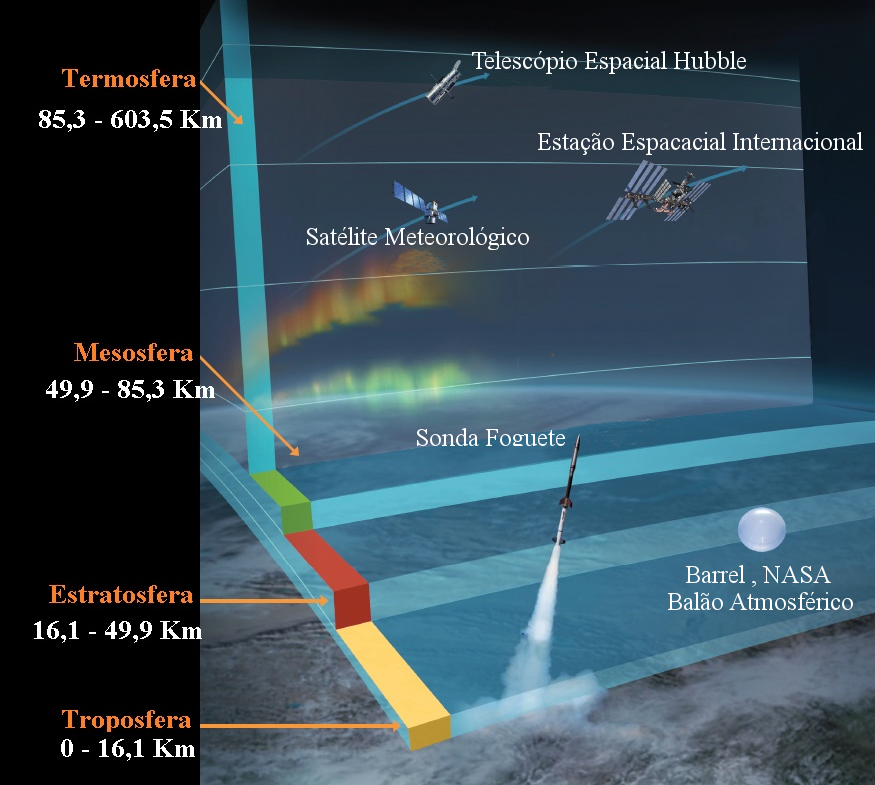
\includegraphics[width=12cm]{figuras/sondas}}
% 		}{
% 			\Fonte{adaptado de \citeonline{NASA2016}.}}	
% 	\end{figure}

%     Texto texto texto texto texto texto texto texto texto texto texto texto texto texto texto texto texto texto texto texto texto texto texto texto texto texto texto texto texto texto texto texto texto texto texto texto texto texto texto texto texto texto texto texto texto.

%     Texto texto texto texto texto texto texto texto texto texto texto texto texto texto texto texto texto texto texto texto texto texto texto texto texto texto texto texto texto texto texto texto texto texto texto texto texto texto texto texto texto texto texto texto texto.

%     Texto texto texto texto texto texto texto texto texto texto texto texto texto texto texto texto texto texto texto texto texto texto texto texto texto texto texto texto texto texto texto texto texto texto texto texto texto texto texto texto texto texto texto texto texto.

%     Texto texto texto texto texto texto texto texto texto texto texto texto texto texto texto texto texto texto texto texto texto texto texto texto texto texto texto texto texto texto texto texto texto texto texto texto texto texto texto texto texto texto texto texto texto.

%     Texto texto texto texto texto texto texto texto texto texto texto texto texto texto texto texto texto texto texto texto texto texto texto texto texto texto texto texto texto texto texto texto texto texto texto texto texto texto texto texto texto texto texto texto texto.

%     \section{Inserindo tabelas}
%     \label{sec:tabelas}

% 	A Tabela \ref{tab:exemplo-1} Texto texto texto texto texto texto texto texto texto texto texto texto texto texto texto texto texto texto texto. Texto texto texto texto texto texto texto texto texto texto texto texto texto texto texto texto texto texto texto.

% \subsection{Exemplo de subseção} \label{sec:ex_sec}
	
% Texto texto texto texto texto texto texto texto texto texto texto texto texto texto texto texto texto texto texto texto texto texto texto texto texto texto texto texto texto texto texto texto texto texto texto texto texto texto texto texto texto texto texto texto texto.

% %acrlong{DATASUS},\acrlong{DNV},\acrlong{DO},\acrlong{ESF},\acrlong{IBGE},\acrlong{MFC},\acrlong{MI},\acrlong{MS},\acrlong{NV},\acrlong{ODM},\acrlong{OI},\acrlong{OMS},\acrlong{ONU},\acrlong{PNI},\acrlong{PSF},\acrlong{RIPSA},\acrlong{RN},\acrlong{SIM},\acrlong{SINASC},\acrlong{SUS},\acrlong{TMI},\acrlong{TMMFC}


% \begin{alineascomponto}
% 	\item Integer non lacinia magna. Aenean tempor lorem tellus, non sodales nisl commodo ut
% 	\item Proin mattis placerat risus sit amet laoreet. Praesent sapien arcu, maximus ac fringilla efficitur, vulputate faucibus sem. Donec aliquet velit eros, sit amet elementum dolor pharetra eget
% 	\item Integer eget mattis libero. Praesent ex velit, pulvinar at massa vel, fermentum dictum mauris. Ut feugiat accumsan augue, et ultrices ipsum euismod vitae
% 	\begin{subalineascomponto}
% 		\item Integer non lacinia magna. Aenean tempor lorem tellus, non sodales nisl commodo ut
% 		\item Proin mattis placerat risus sit amet laoreet.
% 	\end{subalineascomponto}
% \end{alineascomponto}

% Teste de siglas \gls{TMMFC}